\documentclass[tikz,border=10pt]{standalone}
\usetikzlibrary{arrows.meta, positioning, calc, decorations.pathreplacing}
\usepackage{amsmath}
\usepackage{amssymb}

\begin{document}
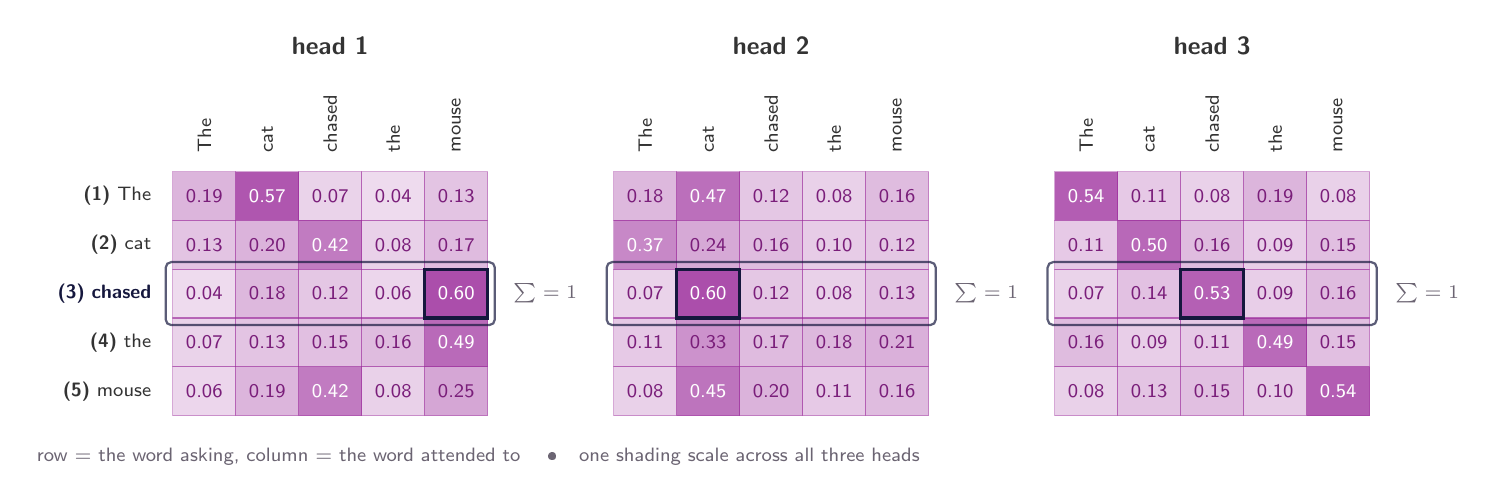
\begin{tikzpicture}[
    every node/.style={font=\sffamily},
]

\definecolor{c1}{HTML}{15173D}   % structure: the frame around row (3)
\definecolor{c2}{HTML}{982598}   % the weights
\definecolor{c3}{HTML}{E491C9}
\definecolor{c4}{HTML}{F1E9E9}
\definecolor{axiscolor}{HTML}{333333}
\definecolor{labelcolor}{HTML}{6B6472}

\def\cw{0.80}   % cell width
\def\ch{0.62}   % cell height

% ================================================================
% Three 5x5 weight tables for "The cat chased the mouse".
% Rows = the querying word, columns = the word attended to.
%
%   head 1  left edge x = 0.00     (the table of section 05, unchanged)
%   head 2  left edge x = 5.60
%   head 3  left edge x = 11.20
% Each table: top edge y = 0, row r spans y in [-(r+1)*ch, -r*ch],
% column c spans x in [c*cw, (c+1)*cw]. Table is 4.00 x 3.10.
%
% y = 1.60   head label
% y = 0.12   column words, rotated 90
% y = -3.55  reading note
% x = -0.15  row words, anchor east
%
% One shared intensity scale for all three tables, identical to the
% weight panel of attention_pipeline: opacity = 0.12 + 1.15*w.
% Row (3) "chased" carries a navy frame in all three; inside it, the
% single cell that takes most of the row carries a heavier navy outline.
% ================================================================

\newcommand{\headtable}[4]{%  #1 x shift, #2 label, #3 peak column, #4 rows
\begin{scope}[shift={(#1,0)}]
  \node[font=\sffamily\small\bfseries, text=axiscolor] at (2.0, 1.60) {#2};

  \foreach \row/\r in #4 {
    \foreach \v [count=\c from 0] in \row {
      \pgfmathsetmacro{\op}{0.12 + 1.15*\v}
      \fill[c2, opacity=\op] (\c*\cw, -\r*\ch-\ch) rectangle ++(\cw, \ch);
      \draw[c2, opacity=0.4, line width=0.4pt]
          (\c*\cw, -\r*\ch-\ch) rectangle ++(\cw, \ch);
      % dark fills need light numerals
      \pgfmathsetmacro{\vv}{\v}
      \ifdim\vv pt>0.35pt \colorlet{celltext}{white}
      \else \colorlet{celltext}{c2!80!black}\fi
      \node[font=\sffamily\scriptsize, text=celltext]
          at (\c*\cw+0.5*\cw, -\r*\ch-0.5*\ch) {\v};
    }
  }

  % the one row every head is compared on
  \draw[c1, opacity=0.70, line width=0.8pt, rounded corners=2pt]
      (-0.09, -3*\ch-0.09) rectangle (4.09, -2*\ch+0.09);
  \node[font=\sffamily\scriptsize, text=labelcolor, anchor=west]
      at (4.20, -2.5*\ch) {$\textstyle\sum = 1$};

  % where that row actually spends its budget
  \draw[c1, line width=1.2pt]
      (#3*\cw, -3*\ch) rectangle ++(\cw, \ch);

  % column words
  \foreach \w [count=\c from 0] in {The, cat, chased, the, mouse} {
    \node[font=\sffamily\scriptsize, text=axiscolor, anchor=west, rotate=90]
        at (\c*\cw+0.5*\cw, 0.12) {\w};
  }
\end{scope}}

\headtable{0.00}{head 1}{4}{{%
    {0.19,0.57,0.07,0.04,0.13}/0,
    {0.13,0.20,0.42,0.08,0.17}/1,
    {0.04,0.18,0.12,0.06,0.60}/2,
    {0.07,0.13,0.15,0.16,0.49}/3,
    {0.06,0.19,0.42,0.08,0.25}/4}}

\headtable{5.60}{head 2}{1}{{%
    {0.18,0.47,0.12,0.08,0.16}/0,
    {0.37,0.24,0.16,0.10,0.12}/1,
    {0.07,0.60,0.12,0.08,0.13}/2,
    {0.11,0.33,0.17,0.18,0.21}/3,
    {0.08,0.45,0.20,0.11,0.16}/4}}

\headtable{11.20}{head 3}{2}{{%
    {0.54,0.11,0.08,0.19,0.08}/0,
    {0.11,0.50,0.16,0.09,0.15}/1,
    {0.07,0.14,0.53,0.09,0.16}/2,
    {0.16,0.09,0.11,0.49,0.15}/3,
    {0.08,0.13,0.15,0.10,0.54}/4}}

% ---------------------------------------------------------------- row words
\foreach \w/\r/\col in {{\textbf{(1)} The}/0/axiscolor, {\textbf{(2)} cat}/1/axiscolor,
                   {\textbf{(3)} \textbf{chased}}/2/c1, {\textbf{(4)} the}/3/axiscolor,
                   {\textbf{(5)} mouse}/4/axiscolor} {
  \node[font=\sffamily\scriptsize, text=\col, anchor=east]
      at (-0.15, -\r*\ch-0.5*\ch) {\w};
}

% ---------------------------------------------------------------- reading note
\node[font=\sffamily\scriptsize, text=labelcolor, anchor=west] at (-1.85, -3.62)
    {row $=$ the word asking, column $=$ the word attended to
     \quad\textbullet\quad one shading scale across all three heads};

\end{tikzpicture}
\end{document}
